\documentclass{article}
% add graphics
\usepackage{graphicx}
% add color
\usepackage{xcolor}
\usepackage{textcomp}
\usepackage{clock}
%\pagecolor[rgb]{0,0,0} %black
%\color[rgb]{0.95,0.95,0.95} %grey
% add links
\usepackage{hyperref}
\usepackage{nopageno}
\usepackage[symbol]{footmisc}
\usepackage{float}
\begin{document}
\title{Diffusion Local Time: hard~real-time multilingual data visualization via multimodal-LLM generative~AI on heterogeneous edge devices for extremely high-impact chronometry and extremely low-cost neurological diagnostics}
\author{\href{mailto:leebutterman@gmail.com}{Lee Steven Butterman}, Poeta ex Machina Labs\\Dr.~Benjamin Forest Fredericks, Developmental Studies, Toad Hall}
\date{}
\maketitle
\begin{abstract}

    \textit{Diffusion Local Time} is the forefront of clock face technology, and solves the tyranny and the tedium of high-visibility low-computation low-power timekeeping like the household clock.

    Through the use of Stable Diffusion 1.5, steered by a ControlNet, the clock face is a customizable generative AI image that renders the hours and minutes of the time with the clarity of spotting faces in clouds, relying on the viewer's pareidolia for them to read the time. % Sometimes, things that are expensive, are worse.

    \textit{Diffusion Local Time} lives in a place between 1) Christian Marclay's \textit{The Clock}, a 24-hour film that is a montage of thousands of film and television images of clocks, edited together so that they show the actual time; 2) \texttt{xdaliclock}, a graphics-intensive timepiece based on a Mac 128K application, where digits morph into each other; 3) digital wristwatches, which are a pretty neat idea.

    The code is at \url{https://github.com/lsb/diffusion-local-time}, and runs on everything from powerful GPUs to small Raspberry Pis.

\end{abstract}

\begin{figure}[H]
    \centering
    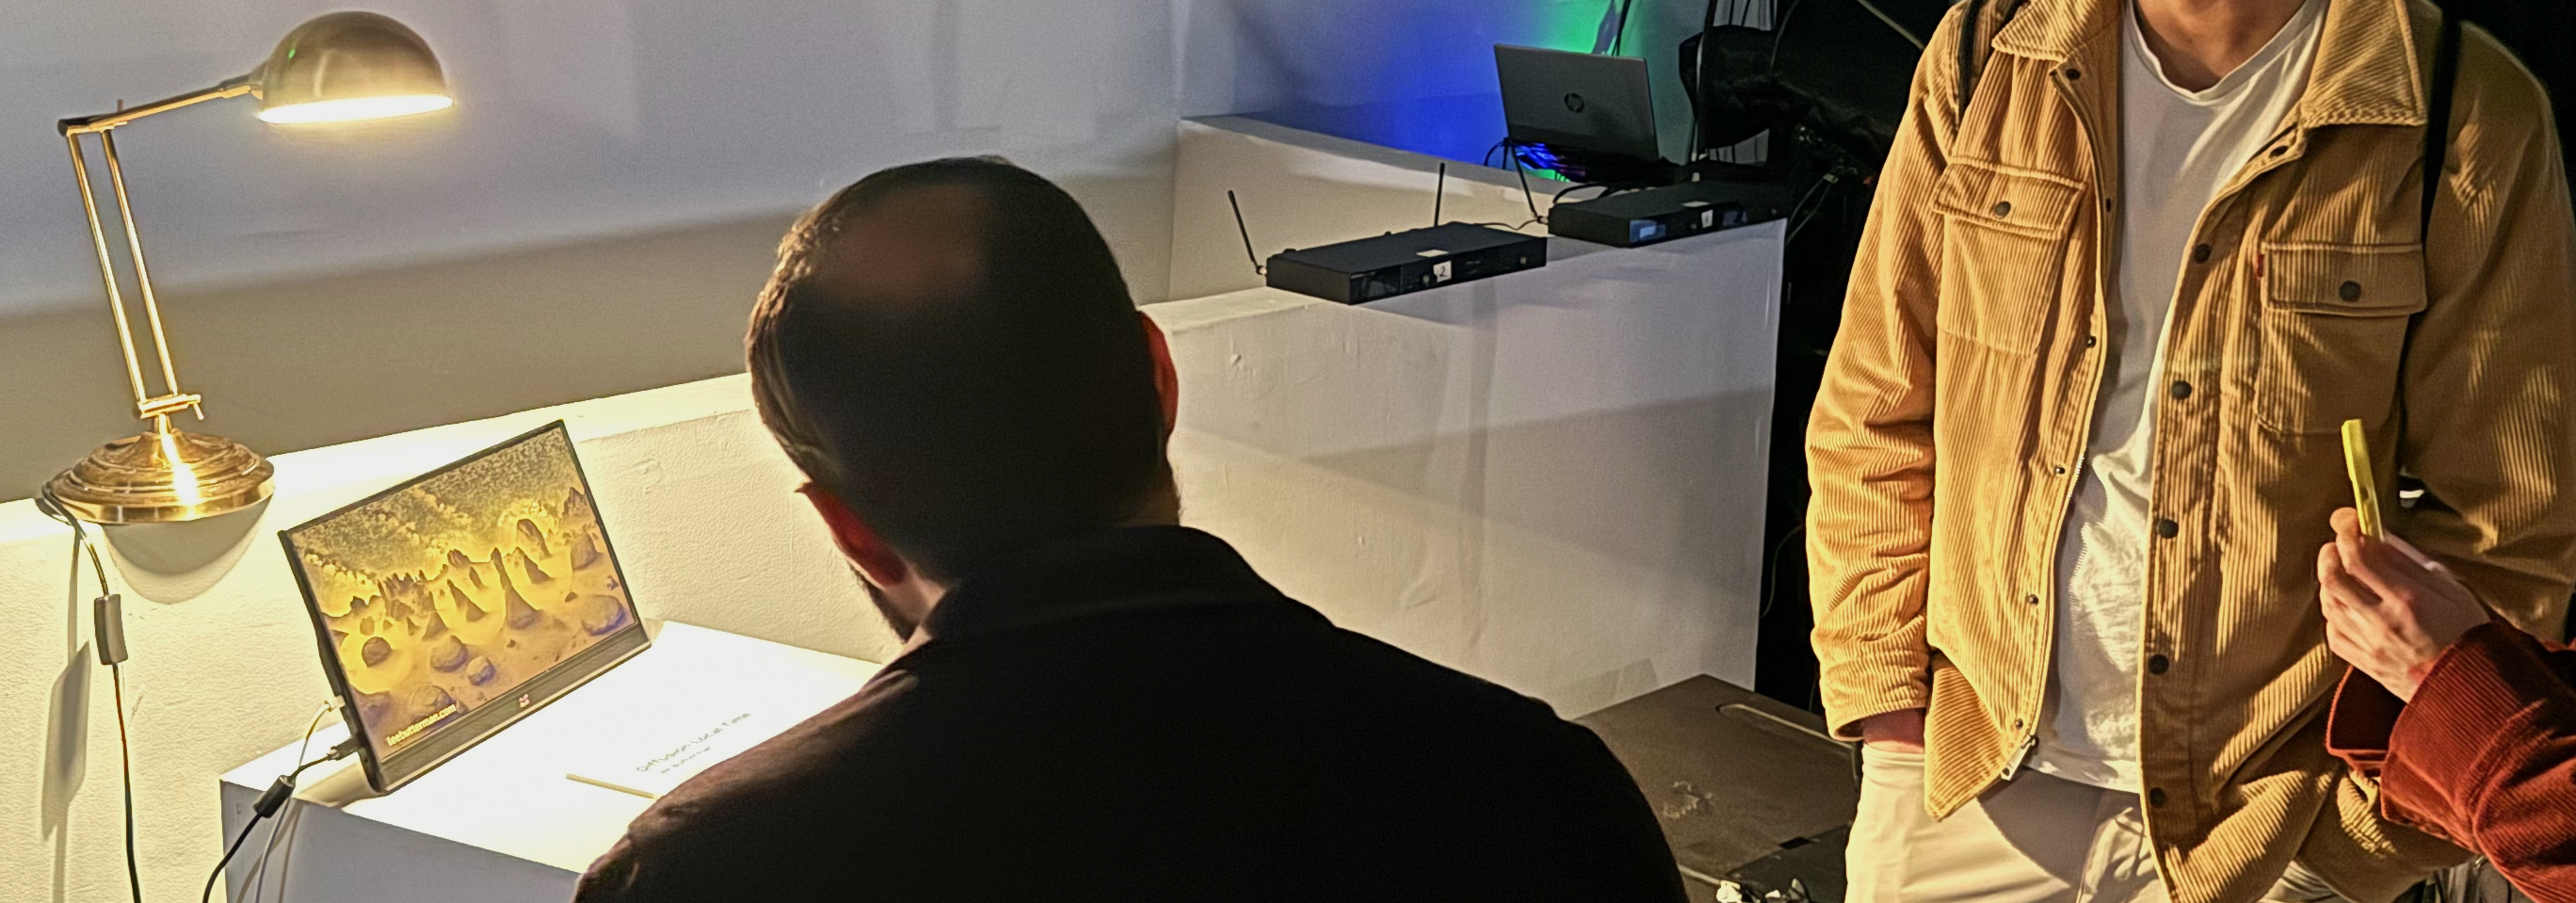
\includegraphics[height=1.5in]{8pm}
    \caption{8:00 PM, as rendered by \textit{Diffusion Local Time}.}
    \label{fig:8pm}
\end{figure}

\pagebreak

\begin{figure}[H]
    \centering
    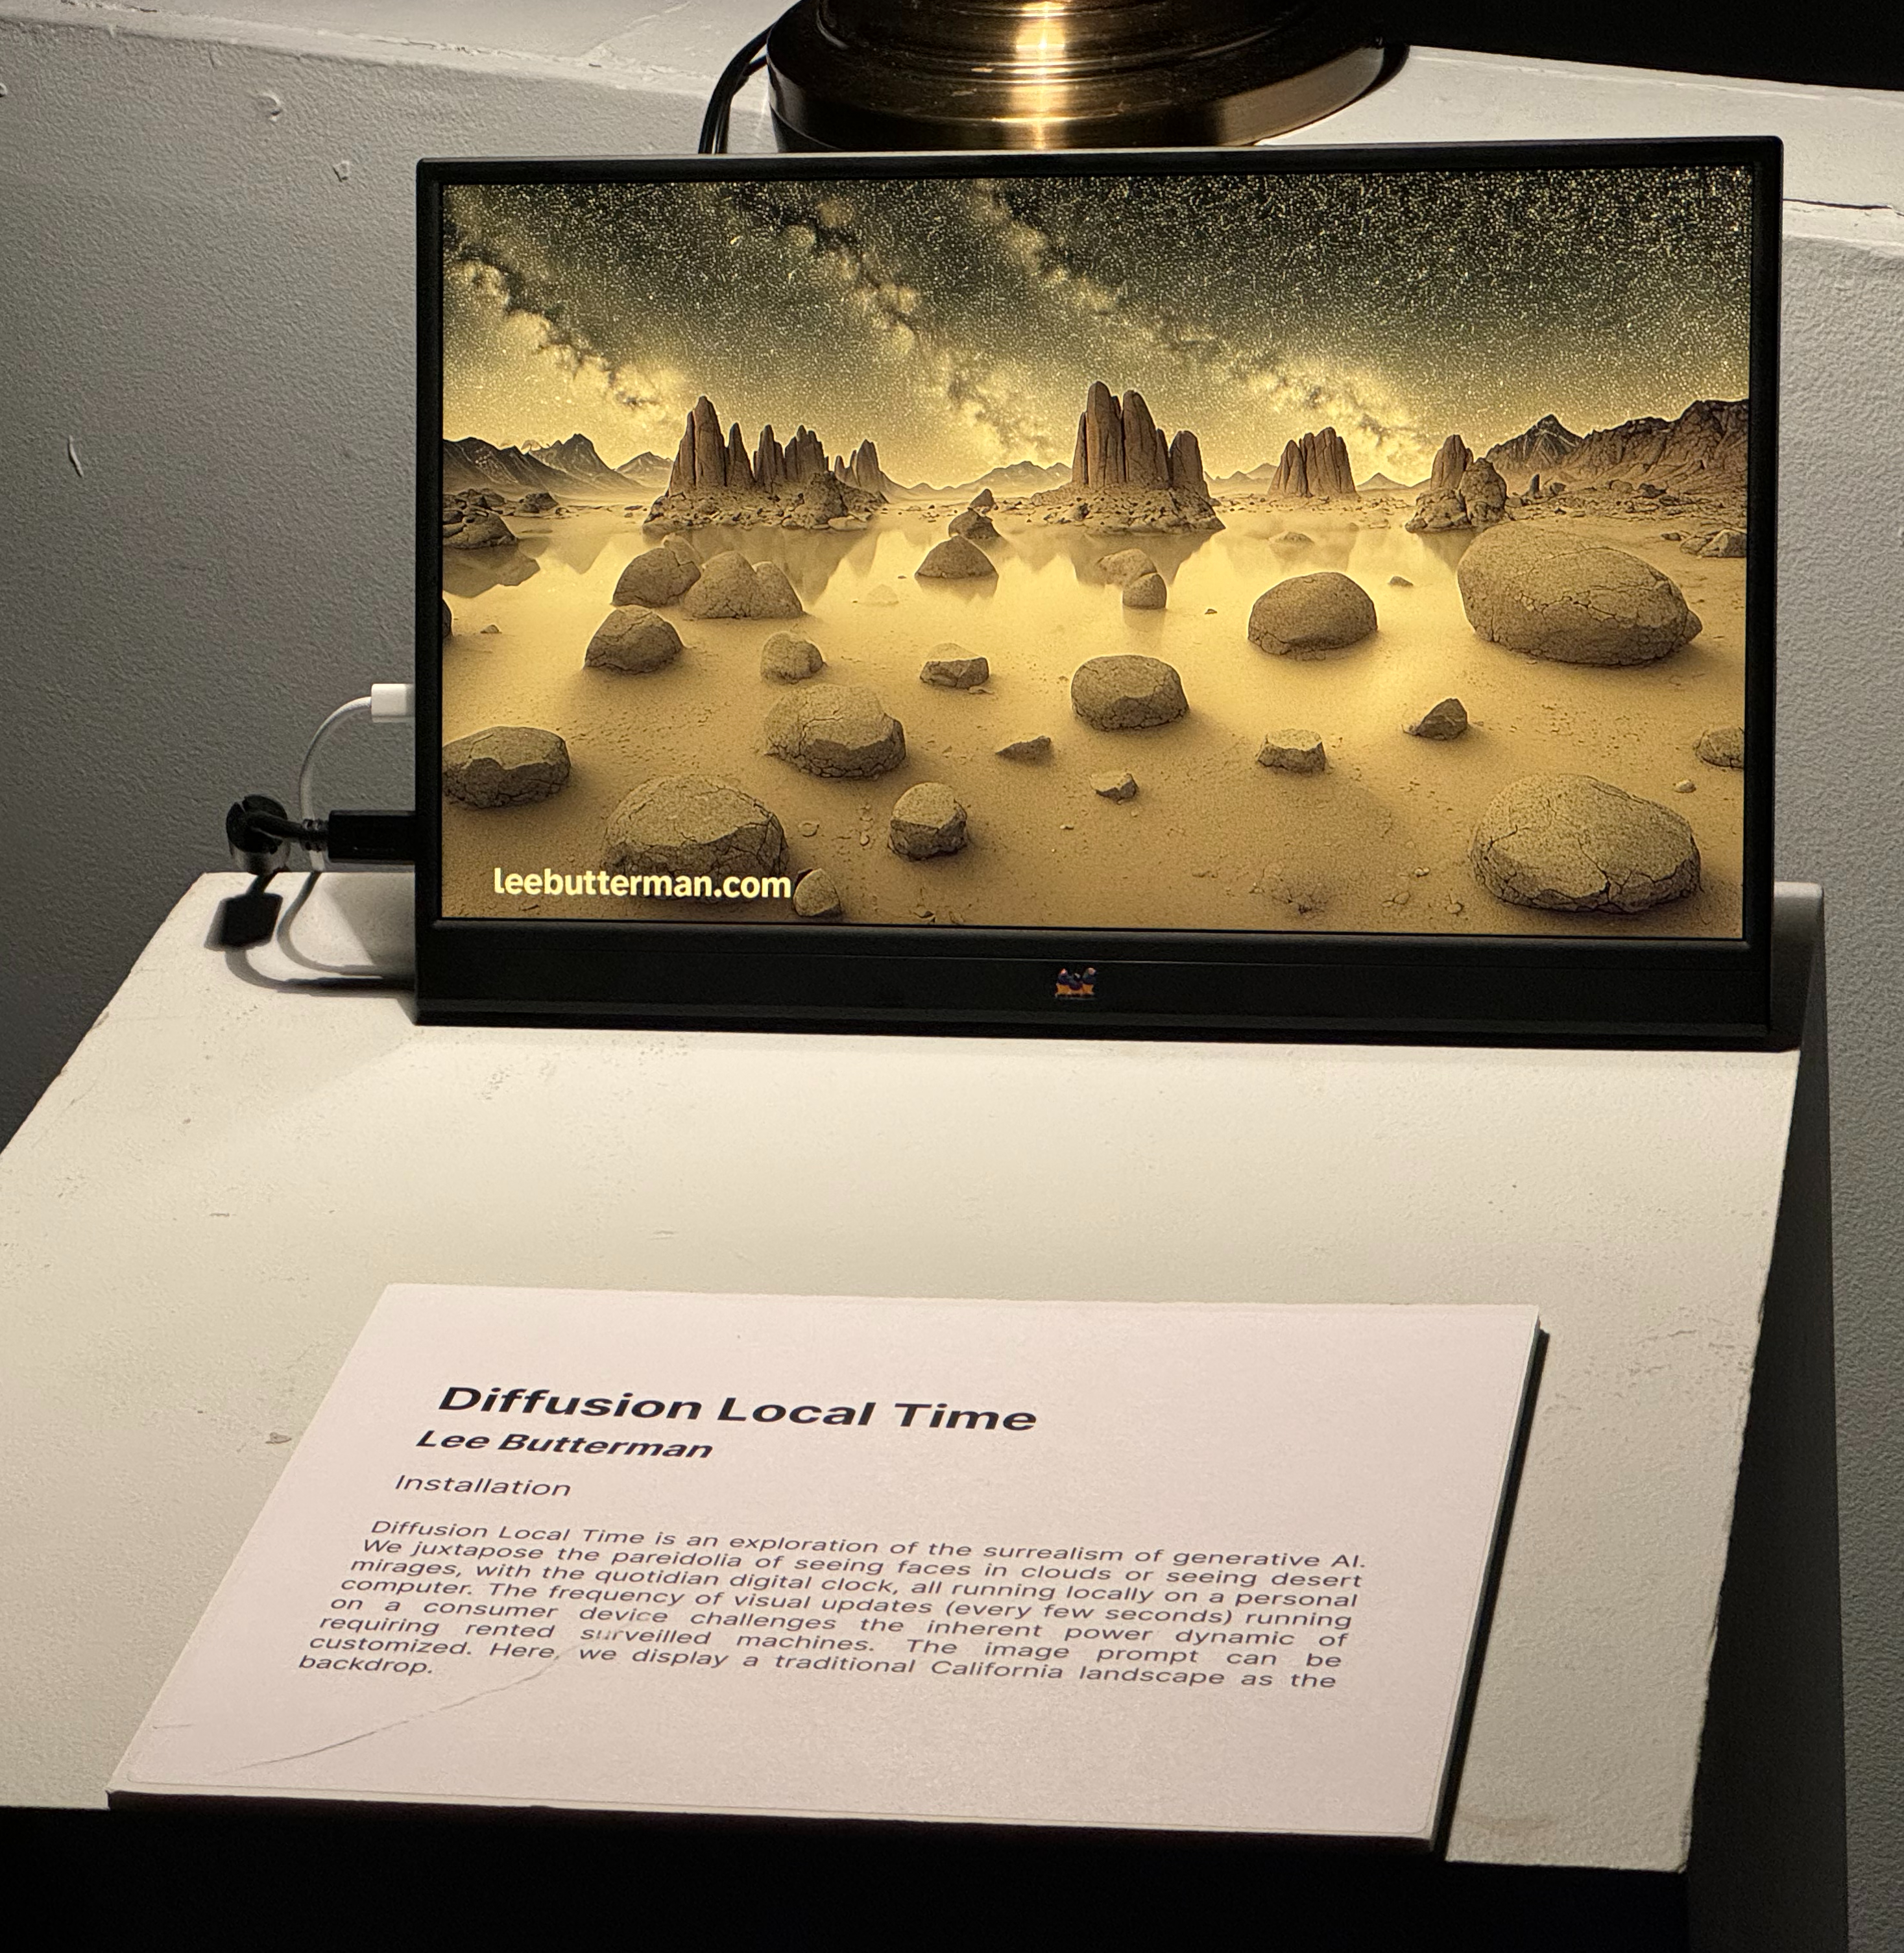
\includegraphics[width=\textwidth]{748}
    \caption{7:48 PM. Note that the legibility changes based on proximity.}
    \label{fig:748}
\end{figure}

\section{Introduction}

Stable Diffusion 1.5 [SD1.5] is a text-to-image model based on diffusion techniques.
Stable Diffusion decomposes the problem of formulating an image into a sequence of denoising steps, often 50 or more. It is possible to distill the denoising trajectory into a Latent Consistency Model [LCM], which can render a high-quality image into only 4 steps or fewer. 
The output is conditioned by a prompt, and can also be steered by an additional ControlNet [ControlNet] model, which impacts the denoising steps.

The control image can be any learnable value per pixel: object depth in the scene to render, object edges, or pixel brightness. Controlling pixel luminance enables generating photorealistic imagery with a subtext, like barcodes, or QR codes [NHCIAO], or promotional materials, as in Figure~\ref{fig:sigboviksunrise}.

\begin{figure}[H]
    \centering
    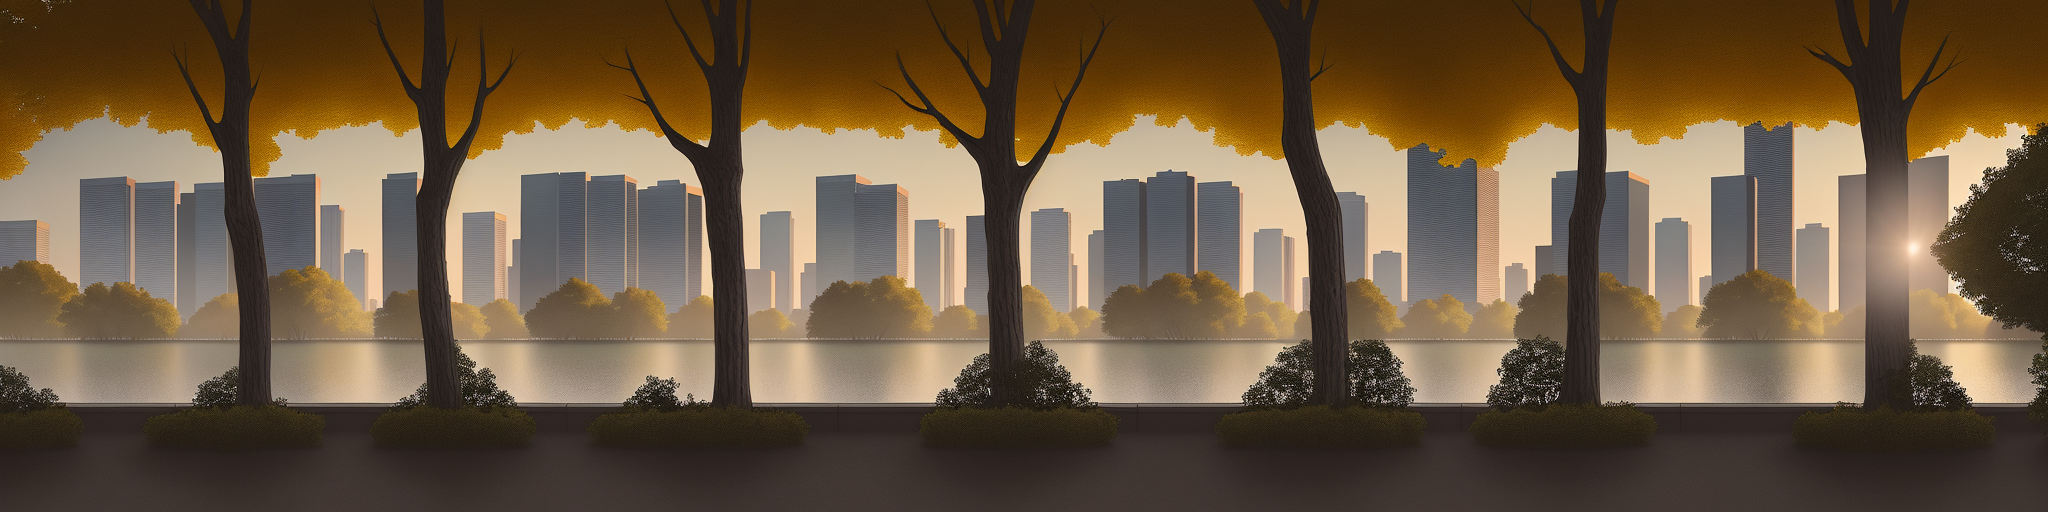
\includegraphics[width=\textwidth]{sigbovik-park-sunrise}
    \caption{A leafy park at sunrise in a large bustling city with tall buildings.}
    \label{fig:sigboviksunrise}
\end{figure}

The readability relies on the viewer's imagination through pareidolia, so typographical choices are crucial for the project's usefulness. The typeface is Atkinson Hyperlegible [Atkinson], which is ``designed to focus on letterform distinction to increase character recognition, ultimately improving readability.''

The legibility of the numeric time is a function of many variables: the prompt, the size of the image, the target distance from the viewer, the strength of the control, and the rest of the scene being rendered for a particular initial noise pattern. When changing the imagery, or the size of the image (based on hardware speeds), it can be useful to do a manual grid search of control strengths and find a strength that generates aesthetically pleasing images that are legible, like in Figure~\ref{fig:8000to1}. Larger images allow for greater flexibility to find plausible objects in a scene for a prompt, so for a certain legibility, choosing a smaller images implies that the mean controlnet conditioning strength would be higher, and the variance would be higher as well, as in Figure~\ref{fig:8000to1480x270}.

\begin{figure}
    \centering
    \includegraphics[height=\textheight]{800-0-to-1}
    \caption{8:00, for ControlNet conditioning strengths from 0.0 to 1.0, for six different random seeds, at size 1440$\times$810. Note that strengths around 0.45 uniformly balance legibility and aesthetics for most seeds.}
    \label{fig:8000to1}
\end{figure}

\begin{figure}
    \centering
    \includegraphics[height=\textheight]{800-0-to-1-480x270}
    \caption{8:00, for ControlNet conditioning strengths from 0.0 to 1.0, for six different random seeds, at size 480$\times$270. Strengths around 0.7 for many of the seeds are optimal, but image plausibility has declined for a legible image, and the variance between seeds for legibility at a particular strength is higher.}
    \label{fig:8000to1480x270}
\end{figure}

The time is displayed as a slideshow, with each image displayed until the next is ready. We achieve consistency of landscapes through keeping identical seeds for image generation, and changing seeds for aesthetic variety every hour, though this is easily field-servicable, which may be desirable when deployed on faster machines.

\section{Costs}

\subsection{Bill of Materials}

\begin{itemize}
    \item Raspberry Pi 5: \$80
    \item 32GB $\mu$SD Card: \$10
    \item 1920x1080 HDMI Monitor: \$110
    \item Optional: NVIDIA DGX A100: \$127,215 MSRP
    \item Optional: IKEA Tromma clock with hour and minute hands: \$2.99
\end{itemize}

\subsection{Power}

A small screen consumes 8W of power, and a Raspberry Pi under load consumes 12W. A wall clock might consume 1 AA/year, which is 4Wh per 525600 minutes [Larson], or 7.6$\mu$W. This artwork thus has 2-3 million times the power and impact of a household clock. Upgrading to a DGX 4xA100, which can render \textit{Diffusion Local Time} animations in realtime, can consume up to 1500W, at 200 million times the impact and power of a household clock, at only 40 thousand times the cost. The more you buy the more you save. [Huang]

%FIXME: after the first write up, and after initial gags, compile SD 1.5 via TVM onto Raspberry Pi 5


\section{Related Work}

\subsection{Steve Capps' and Jamie Zawinski's \textit{Dali Clock}}

\begin{figure}[H]
    \centering
    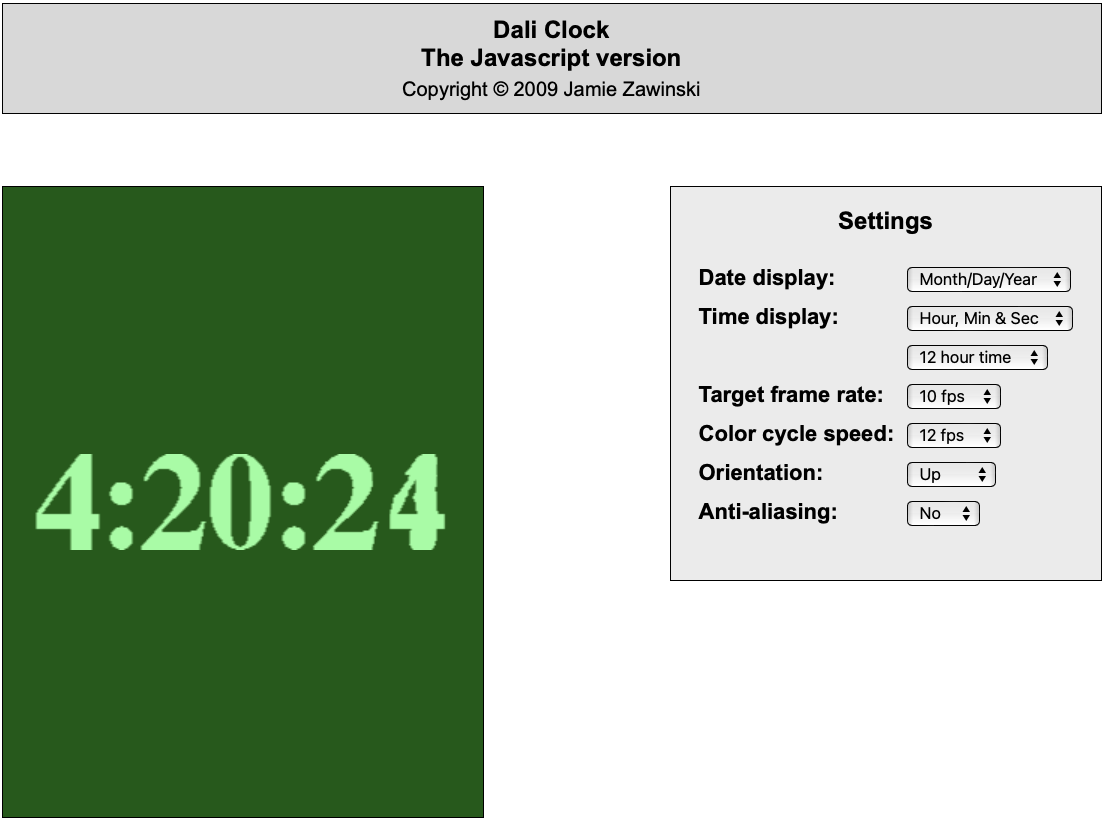
\includegraphics[width=2in]{daliclock42024}
    \caption{The \texttt{xdaliclock} application, in Javascript.}
    \label{fig:daliclockjwz}
\end{figure}

The \textit{Dali Clock} is a graphics-intensive timepiece, created originally by Steve Capps for the Xerox Alto and then rewritten for the Mac 128K, and then rewritten by Jamie Zawinski for XWindows  as \texttt{xdaliclock} and also for web browsers in Javascript. The animation is smooth, even on a 7 MHz Mac 128K computer, morphing digits from second to second in HH:MM:SS format. The typography is relatively fixed, and the background color changes slowly over time.

On a modern consumer desktop, rendering a 1600x900 image can take multiple seconds on a GPU. However, the original deploy target of the Alto launched in 1973 and initially cost \$32k, equivalent to \$233k in 2022. This price is almost the cost of two NVIDIA DGX 4xA100 boxs at MSRP, \$130k in March 2024.  On a DGX, currently, it would be possible to create a variation, with seconds included, to render an animataion at dozens of frames per second at relatively high resolution, in the style of the Dali Clock.

For enthusiasts of the Dali Clock with a spare DGX, we share a few seconds of 30 fps animation stills in Figures \ref{fig:xdalidlt0} and \ref{fig:xdalidlt1}.

\begin{figure}
    \centering
    \includegraphics[height=\textheight]{0000dali}
    \caption{The 12:00:00AM second of \textit{Diffusion Local Time} animation in the style of \texttt{xdaliclock}.}
    \label{fig:xdalidlt0}
\end{figure}

\begin{figure}
    \centering
    \includegraphics[height=\textheight]{0001dali}
    \caption{The 12:01:00AM second of \textit{Diffusion Local Time} animation in the style of \texttt{xdaliclock}.}
    \label{fig:xdalidlt1}
\end{figure}

\subsection{Christopher Marclay's \textit{The Clock}}

The Clock is a 24-hour film that is a montage of over ten thousand clips from film and television of clocks, edited together so that they show the actual time. Marclay viewed the film as a memento mori, drawing attention to how much time the audience has spent watching it, compared to the escapism that cinema often provides. [Marclay]

In contrast, \textit{Diffusion Local Time} quickly lets the audience lose themselves in the landscapes, and revels in the escapism that is a display that quite literally disappears on close inspection.

Further, \textit{Diffusion Local Time} is field-servicable for the user's own tastes, and the time can optionally be synchronized with networked time servers on startup as needed. Advancements in text-to-video technology [Sora] make one hopeful that a future version of \textit{The Clock} will be able to be generated on the fly, and be able to be customized to the user's tastes.

\subsection{Digital wristwatches: a pretty neat idea}

Digital watches came along at a time that, in other areas, we were trying to find ways of translating purely numeric data into graphic form so that the information leapt easily to the eye. For instance, we noticed that pie charts and bar graphs often told us more about the relationships between things than tables of numbers did. So we worked hard to make our computers capable of translating numbers into graphic displays. At the same time, we each had the world's most perfect pie chart machines strapped to our wrists, which we could read at a glance, and we suddenly got terribly excited at the idea of translating them back into numeric data, simply because we suddenly had the technology to do it. Compare \ClockStyle=3\ClockFrametrue\clock{15}{39} to \textbf{{15:39}}, especially in situations where seconds count at odd times, like internet flash sales, or flying commercial. [AdamsPreiss]

\section{Diagnostic Usage}

\textit{Diffusion Local Time} relies on the viewer to intuit the visual illusion to recognize the time, and will usually display a wave of enthusiastic recognition when they perceive what is going on. The underlying technology of the particular StableDiffusion ControlNet can be used to help in neurological diagnostics.

\subsection{Pareidolia}

Pareidolia is commonly associated with seeing faces in clouds, imposing a meaningful interpretation on a nebulous stimulus. It is well established that part of the brain that recognizes faces can also activate when the brain recognizes novel objects like `greebles' [Gauthier], and literacy is widespread in many nations, leading to the possibility of pareidolia presenting as seeing text in clouds or inkblots.

Pareidolias do not reflect visual hallucinations themselves but may reflect susceptibility to visual hallucinations, and increased hallucinations can be indicative of mild cognitive impairment or dementia. [UchiyamaDLB]

The state of the art is the Pareidolia test, which is a test for dementia with Lewy bodies, where the patient is shown a series of images and asked to identify if they see a face in the image. [MamiyaPT] The test is useful as one small part of a differential diagnosis, but one small problem with the current test is the large difference between positive and negative images, as shown in Figure~\ref{fig:pareidoliatest}.


\begin{figure}
    \centering
    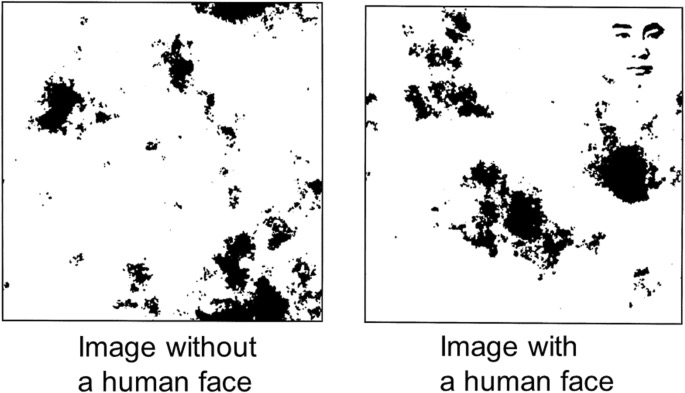
\includegraphics[width=\textwidth]{pareidolia-test-carolyn}
    \caption{Sample image from the current pareidolia test.}
    \label{fig:pareidoliatest}
\end{figure}

\begin{figure}
    \centering
    \texttt{~\\
        SSSSSSSSSSSSSSSSSSSSSSS \\
        SSSSSSSSSSSSSSSSSSSSSSS \\
        SS~~~~~~~SSSSS~~~~~~~SS \\
                  SSSSS           \\
                  SSSSS           \\
%                  SSSSS           \\
                  SSSSS           \\
                  SSSSS           \\
                  SSSSS           \\
                 SSSSSSS          \\
              SSSSSSSSSSS       \\
    }
    \caption{Navon figure.}
    \label{fig:navon}
\end{figure}

\subsection{Simultanagnosia}

Simultanagnosia is a condition where the patient can only perceive one object at a time, and is often tested with Navon figures, where a large letter is composed of smaller letters. This Navon figure is limited by the binary nature of the composition: note that in Figure~\ref{fig:8000to1} the strength of the control can be adjusted, and instead of a binary result from the test a continuous result can be obtained. This can be useful for tracking progression of a patient over time.

Similarly, people who hear voices are much more likely to be able to be conditioned to perceive hallucinations. [Powers] The susceptibility to hallucinations can thus be measured as a continuous variable by the strength of the ControlNet. More research is needed to repeatably calibrate the legibility of the generated images, with optical character recognition or otherwise.

\begin{figure}[H]
    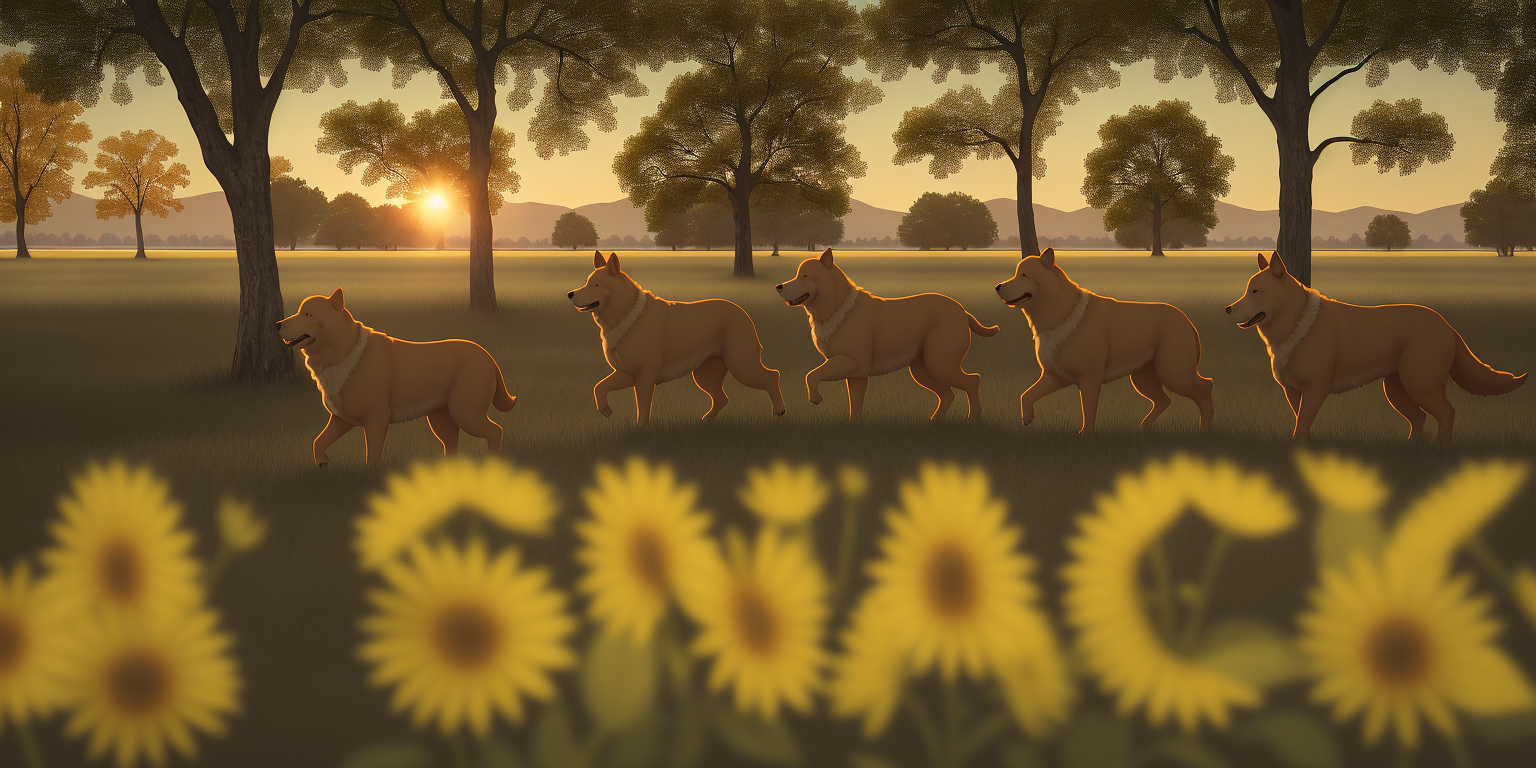
\includegraphics[width=\textwidth]{ask-for-a-snack-corgis}
    %\includegraphics[width=\textwidth]{ask-for-a-snack}
    \caption{Sample image with diagnostic value, when a patient requests a snack.}
    \label{fig:askforasnack}
\end{figure}

\subsection{Future interdisciplinary collaboration}

Future work includes an interdisciplinary collaboration between Neuroscience, Facilites Management's Art Department subdivision, and Catering Services, to redecorate hospital waiting areas with static or dynamic landscapes, to allow patients to experience a generative AI image that is designed to provoke a comment to staff.

Small shelf-stable juice boxes of common beverages like apple juice or water, and small sachets of common food items like graham crackers or almonds, can be concealed nearby for easy distribution in the waiting area, and the patient's request can be recorded in their chart for potential diagnostic value. These items are widely distributed upon request in clinical settings, generally considered healthy, and billable to insurance.




\newpage

\section*{Bibliography}

~\setlength{\parindent}{0pt}\setlength{\parskip}{1em}

AdamsPreiss: Douglas Adams, fax with Byron Preiss, 1992, as quoted in \textit{The Ultimate Hitchhiker's Guide to the Galaxy} and excerpted in \href{https://web.archive.org/web/20230330020214/https://lettersofnote.com/2023/02/11/please-dont-let-anyone-americanise-it/}{\textit{Letters of Note}}.

Atkinson: Braille Institute. Atkinson Hyperlegible Font. \url{https://www.brailleinstitute.org/freefont}

ControlNet: Lvmin Zhang, Anyi Rao, Maneesh Agrawala. Adding Conditional Control to Text-to-Image Diffusion Models. \url{https://arxiv.org/abs/2302.05543}

Gauthier: I Gauthier, M J Tarr, A W Anderson, P Skudlarski, J C Gore. Activation of the middle fusiform 'face area' increases with expertise in recognizing novel objects. Nat Neurosci. 1999 Jun;2(6):568-73. doi: 10.1038/9224. PMID: 10448223.

Huang: Jensen Huang, \href{https://s201.q4cdn.com/141608511/files/doc_presentations/2018/04/JHH_GTC2018_FINAL_PRESENTED_16X9.pdf}{personal communication}, 27 March 2018.

Larson: Jonathan Larson. Rent. 1996.

LCM: Simian Luo, Yiqin Tan, Longbo Huang, Jian Li, Hang Zhao. Latent Consistency Models: Synthesizing High-Resolution Images with Few-Step Inference. \url{https://arxiv.org/abs/2310.04378}

MamiyaPT: Yasuyuki Mamiya, Yoshiyuki Nishio, Hiroyuki Watanabe, Kayoko Yokoi, Makoto Uchiyama, Toru Baba, Osamu Iizuka, Shigenori Kanno, Naoto Kamimura, Hiroaki Kazui, Mamoru Hashimoto, Manabu Ikeda, Chieko Takeshita, Tatsuo Shimomura, and Etsuro Mori. The Pareidolia Test: A Simple Neuropsychological Test Measuring Visual Hallucination-Like Illusions. \url{https://www.ncbi.nlm.nih.gov/pmc/articles/PMC4865118/}

Marclay: Christian Marclay. The Clock. \url{https://www.tate.org.uk/whats-on/tate-modern/exhibition/christian-marclay-clock}

NHCIAO: Benj Edwards. Redditor creates working anime QR codes using Stable Diffusion. \url{https://arstechnica.com/information-technology/2023/06/redditor-creates-working-anime-qr-codes-using-stable-diffusion/}

Powers: A R Powers, C Mathys, P R Corlett. Pavlovian conditioning-induced hallucinations result from overweighting of perceptual priors. Science. 2017 Mar 31;355(6302):596-600. doi: 10.1126/science.aan3458. PMID: 28360244; PMCID: PMC5481463.

SD1.5: Robin Rombach, Andreas Blattmann, Dominik Lorenz, Patrick Esser, Bj\"orn Ommer. High-Resolution Image Synthesis With Latent Diffusion Models. \url{https://arxiv.org/abs/2112.10752}

Sora: Tim Brooks and Bill Peebles and Connor Holmes and Will DePue and Yufei Guo and Li Jing and David Schnurr and Joe Taylor and Troy Luhman and Eric Luhman and Clarence Ng and Ricky Wang and Aditya Ramesh. Video generation models as world simulators. \url{https://openai.com/research/video-generation-models-as-world-simulators}

UchiyamaDLB: Makoto Uchiyama, Yoshiyuki Nishio, Kayoko Yokoi, Kazumi Hirayama, Toru Imamura, Tatsuo Shimomura, Etsuro Mori. Pareidolias: complex visual illusions in dementia with Lewy bodies. \url{https://www.ncbi.nlm.nih.gov/pmc/articles/PMC3407420/}

XDali: Jamie Zawinski. \texttt{xdaliclock}. \url{https://www.jwz.org/xdaliclock/}

\end{document}
